\documentclass[11pt]{article}

\textwidth 17cm
\textheight 23cm
\oddsidemargin 0.25cm
\addtolength{\voffset}{-2.4cm}
\addtolength{\hoffset}{-0.5cm}

\setlength{\parindent}{12pt}
\setlength{\parskip}{3pt}
\usepackage{float, comment}

%\usepackage{refcheck}

%\usepackage[caption = false]{subfig}

\usepackage{amssymb,amsmath,epsfig}

%\usepackage[colorlinks=true,breaklinks=true,linkcolor=black,citecolor=black]{hyperref}

\usepackage{graphics,psfrag,graphicx,color,float,subcaption} %amsthm

\numberwithin{equation}{section}
\numberwithin{figure}{section}

\usepackage[table]{xcolor}

% OUR DEFINITIONS %%%%%%%%%%%%%%%%%%%%%%%%%%%%%%%%%%%
\usepackage{sebastyle}
\DeclareMathAlphabet\mathbfcal{OMS}{cmsy}{b}{n}

\newcommand{\rred}[1]{\textcolor{red}{#1}}
\newcommand{\ccite}{\rred{****CITE HERE****}}
% END OF OUR DEFINITIONS %%%%%%%%%%%%%%%%%%%%%%%%%%%%%

%\allowdisplaybreaks

%***********************************************************************************

\title{New techniques and technologies in data driven approaches to sustainability
\thanks{This research was 
partially supported by  Pacific Institute for the Mathematical Sciences, Mitacs, QuanSight, West Grid and Cybera.}}

\author{{\sc Edgar Pacheco}\thanks{Department of Mathematics and Statistics, University of Calgary, Canada.
email: {\tt edgar.pachecocastan@ucalgary.ca}.}
\and
{\sc Symon Islam}\thanks{Department of ...
email: {\tt your email}.}
\and
{\sc Thomas Pender}\thanks{Department of Mathematics and Computer Science, University of Lethbridge, Canada.
email: {\tt thomas.pender@uleth.ca}.}
\and
{\sc Igor Pinheiro}\thanks{Department of ...
email: {\tt your email}.}
\and
{\sc Sebasti\'an Moraga}\thanks{ Department of Mathematics, Simon Fraser University, Canada.
email: {\tt smoragas@sfu.ca}.}}

\date{}

\begin{document}

\maketitle

\begin{abstract}
\noindent
In this paper we propose and analyze [...] In this part we write the possible abstract for the project.

\end{abstract}

\begin{comment}
\noindent
{\bf Key words}: Machine learning, agriculture, climate change, optimization, water
\end{comment}

\smallskip\noindent

                                                  
%%%%%%%%%%%%%%%%%%%%%%%%%%%%%%%%%%%%%%%%%%%%%%%%%%%%%%%%%%%%%%%%%%

\section{Introduction}\label{introduction}

Sustainability is the greatest challenge facing the human race, and in the face of global warming coupled with population increase, the strain on vital sectors, like agriculture, is mounting at an accelerated pace. This project is focused on the use of open data to improve understanding, and, ideally, predictability, for the environmental impact from agriculture. 

Agriculture is one of the most significant areas of economic activity for countries around the world, and it has a significant environmental impact; it is estimated that agriculture accounts for at least $10\%$ of green house gas emissions in many countries \ccite. In nearly every country, there is an impact from agricultural practices through changing land use, water consumption, use of fertilizer, GHG and other emissions. From a local perspective agriculture creates different dynamics for indigenous plant and animal life in addition to creating different micro-climates. On a more broad scale, agriculture can put pressure on entire river systems and lead to changing weather patterns as atmospheric humidity and solar radiation emissions change.

The ideal outcome of this project is the design of a model and a system of action for environmental impacts that leverages open data and provides a complement to the current TheoryMesh system which is capturing operational impacts from farm activities. Invariably, the project and its outcome will be data driven.

There are many data sources available to investigate environmental changes and impacts due to agriculture. Furthermore, there is a proliferation of data sets that convey information about practices, agricultural production, and green house gas emissions. Combining data across data sources and interpreting the data in new ways could provide better insights on sustainability. Using machine learning techniques to creating models to describe these impacts could improve planning and shift practices to reflect longer term environmental impact. For example, technologies like Blockchain may provide a foundation to create an immutable data ledger for environmental impact while also leveraging smart contracts to take action on data when conditions are met.

For a broader view, the reader is encouraged to read The United Nations Sustainable Development Goals that describe a multi-faceted view of sustainability covering environment, economic and societal factors \ccite.

%%%%%%%%%%%%%%%%%%%%%%%%%%%%%%%%%%%%%%%%%%%%%%%%%%%%%%%%%%%%%%%%%%

\section{Problems}\label{problems}

The issues elluded to above are broad, and they are difficult to quantify and to analyze; indeed, agricultural sustainability is a function of a large number of variables. In an effort to make the problem more tractable, we focused on two smaller problems.

The first problem arose in the following way. There is a lot of work being done on the broader, macro scale. However, it is interesting that not much work has been done on the local, micro level. For instance, a common complaint among contemporary farmers is that information cannot be compiled and disseminated in the same ways anymore. It used to be the case that a producer might say ``Plant this crop on this day because that is what has always worked.'' This is no longer tenable with the changing climate and increased weather volatility.

All this is to say that the productivity of agricultural fields, what producers depend on, is being negatively affected, and new approaches to collecting, interpreting, and disseminating relavent information need to be produced.

The second problem ... \rred{SEBASTIAN: What you worked on...}

\subsection{Productivity of Canadian Farms}\label{productivity}

There are many areas in the world that are experiencing the catastrophic effects of climate change. In the Middle East, many of the farmers who have had to rely on local tributaries to sustain their crops are having to to consider different ways of life as water levels of these rivers and lakes decrease and, ultimately, disappear. As these climate events unfold, the UN \ccite warns of a proliferation of conflict over the increase in water scarcity.

For more northern regions, like Canada, the situation may develop differently. As the climate warms, areas to the north will continue to become more viable for a greater variety of agricultural practices and commodities. For instance, consider the length of the frost free days in the province of Alberta \ccite.

In each climate model, as indicated by Figure \ref{ABfrostdays}, the number of consecutive frost free days will invariably increase. With the increased length of the growing season, there will be more opportunities to grow a greater variety of crops in regions that have been hitherto difficult to cultivate.

There are other climate variables to consider as well. Observe the cummulative monthly mean temperature in Alberta over the consecutive frost free days shown in Figure \ref{ABmeantemp} \ccite.

These climate projections per locale can be used by producers in order to project at what points they may profitably consider changes in the location of their business and the type of crops they choose to grow in these locations.

To further evince the increasing productivity of Canadian crop yields, and to provide specific crop data per locale for producers, we can consider data like that shown in Figure \ref{ABbarleyyields}, which shows the change in barley yields in Alberta \ccite. 

Assuming the yield to a be a function time and a number climate variables, say, the number of days with max temperature greater than 32 $^\circ$C, the number of frost free days, the cummulative precipitation, and the cummulative monthly mean temperature, we endevour to use the usual multilinear regression techniques and tools to exterpolate into the future (here we have the popular sklearn module).

As is clear from Figure \ref{ABprojections}, the particular climate model we are assuming has a great effect on the projected yield. We note that rcp26, rcp45, and rcp85 are, respectively, the low, mid, and high emisions models. It is projections such as these that producers may find benificial in making informed choices in a time of increased volatility.

\subsection{\rred{SEBASTIAN'S WORK}}%\label{}

\section{Future Work}

\begin{comment}
\subsection*{Outline}
\MG{Sebastian: Here a little bit of outline of the  project, we  should write this aprt after the main parts are in place.}

\section{Motivation}
\begin{itemize}
\item Bullet points for the main motivation.
\item Should talk about the importance of the model
\item Why does it fit the data.

\item etc.
\end{itemize}
\section{Contributions}
\begin{itemize}
\item Contributions of our work
\item How does our work  (try to-) fix the problem. etc
\end{itemize}
\section{Related work}

\begin{itemize}
\item A little of literature review
\end{itemize}
\section{Setup}

\begin{itemize}
\item Main mathematical setup. All that is needed to  understand the problem.
\MG{Sebastian: Maybe this part changes as we  go  with the project, because should be something more for the industry  than theoretical.}
\end{itemize}
\section{The model problem}

\begin{itemize}
\item What kind of model, prediction are we using. Machine learning approaches, regression models, etc...
\end{itemize}
\section{Problem statement}

\begin{itemize}
\item We should talk a bit of the  statement of the problem 
\end{itemize}
\section{Main results}

\section{Conclusions}

\section{Future work}
\end{comment}
%%%%%%%%%%%%%%%%%%%%%%%%%%%%%%%%%%%%%%%%%%%%%%%%%%%%%%%%%%%%%%%%%%%%%%%%%%%%%%%%%%%%%%%%%%

\begin{thebibliography}{99}

\bibitem{McInn}
{\sc D. McInnes},
Agri-food sustainability targets. A selected overview. DMci Strategies, October 2003.

\bibitem{SMWRA}
{\sc K. Parris},
Sustainable management of water resources in agriculture. OECD Publishing. France, 2010.

 

\end{thebibliography}

\section*{Figures}\label{figures}

\begin{figure}[h!]
\centering
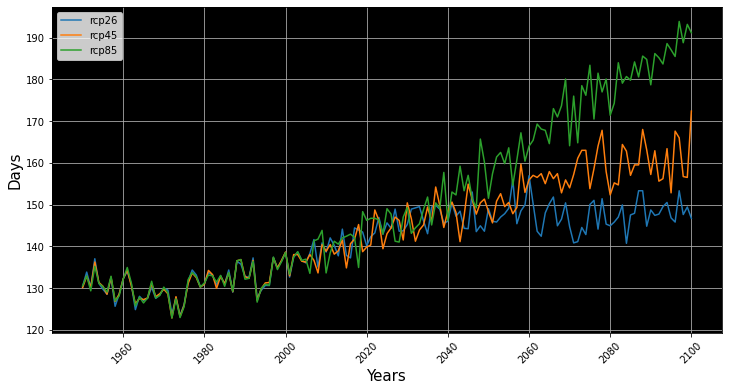
\includegraphics[scale=0.4]{ABfrost}
\caption{Consecutive Frost Free Days in Alberta}
\label{ABfrostdays}
\end{figure}

\begin{figure}[h!]
\centering
 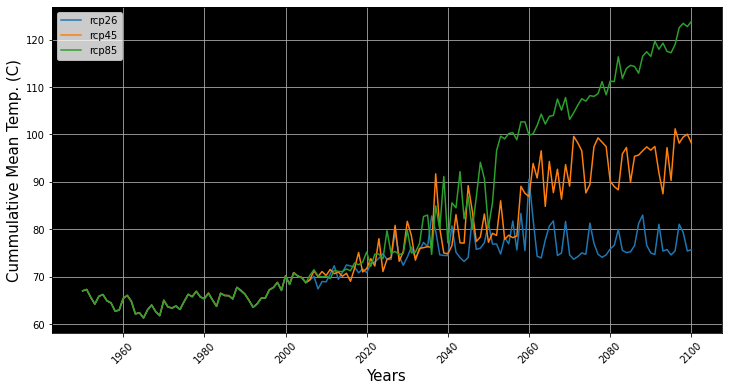
\includegraphics[scale=0.4]{ABtemp}
 \caption{cummulative Mean Temperatures in Alberta}
 \label{ABmeantemp}
\end{figure}

\begin{figure}[h!]
\centering
 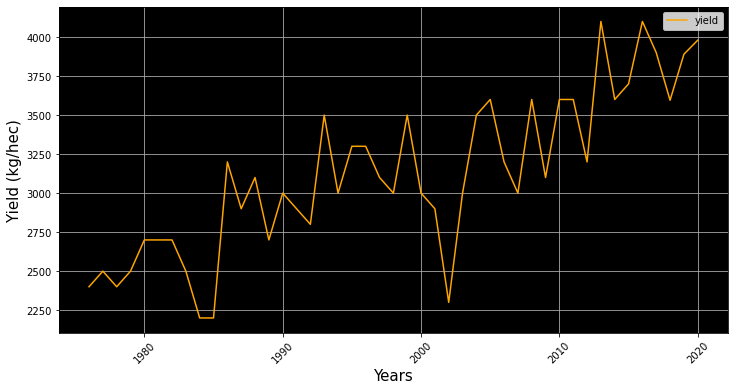
\includegraphics[scale=0.4]{AByield}
 \caption{Barley Yields in Alberta}
 \label{ABbarleyyields}
\end{figure}

\begin{figure}[h!]
 \centering
 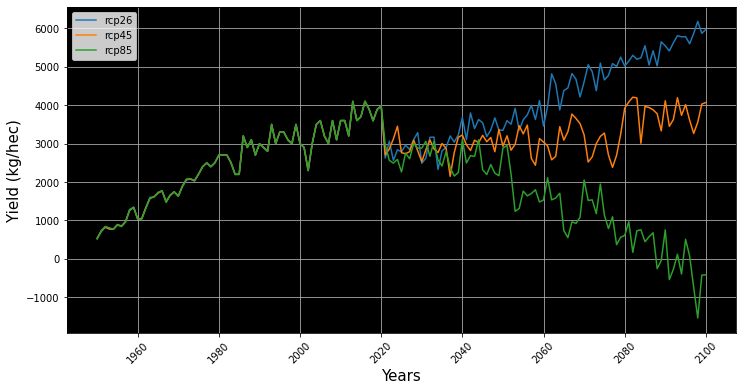
\includegraphics[scale=0.4]{ABproj}
 \caption{Projected Barley Yields in Alberta}
 \label{ABprojections}
\end{figure}


\end{document}

